\begin{frame}{Exemplo 1}
\begin{columns}

\begin{column}[t]{0.38\textwidth}

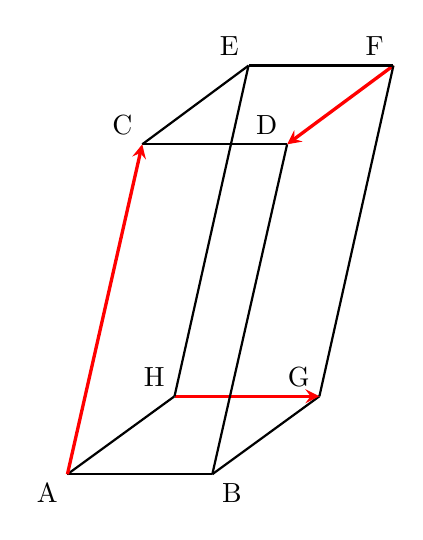
\begin{tikzpicture}[>=stealth]
    \coordinate (A) at (0.35,0.56);
    \coordinate (B) at (2.19,0.56);
    \coordinate (C) at (1.3,4.75);
    \coordinate (D) at (3.14,4.75);
    \coordinate (E) at (2.65,5.75);
    \coordinate (F) at (4.49,5.75);
    \coordinate (G) at (3.55,1.55);
    \coordinate (H) at (1.71,1.55);
    \draw [thick] (A) -- (B);
    \draw [thick] (B) -- (G);
    \draw [very thick, ->, red] (H) -- (G);
    \draw [thick] (H) -- (A);
    \draw [thick] (C) -- (D);
    \draw [very thick, ->, red] (F) -- (D);
    \draw [thick] (F) -- (E);
    \draw [thick] (E) -- (C);
    \draw [very thick,->, red] (A) -- (C);
    \draw [thick] (D) -- (B);
    \draw [thick] (H) -- (E);
    \draw [thick] (F) -- (G);
    \node [below left]  at (A) {A};
    \node [below right] at (B) {B};
    \node [above left]  at (C) {C};
    \node [above left]  at (D) {D};
    \node [above left]  at (E) {E};
    \node [above left]  at (F) {F};
    \node [above left]  at (G) {G};
    \node [above left]  at (H) {H};
\end{tikzpicture}
\end{column}

\begin{column}[t]{0.62\textwidth}
\begin{itemize}
    \item Sejam os vetores \(\vec{AC}\), \(\vec{HG}\) e \(\vec{FD}\)
    \item Vamos calcular \(\vec{AC}+\vec{HG}+\vec{FD}\)
    \item Temos que \(\vec{HG}=\vec{EF}\) (mesma direção, tamanho e sentido)
    \item Temos que \(\vec{AC}=\vec{HE}\) (mesma direção, tamanho e sentido)
\end{itemize}
\end{column}
\end{columns}

\end{frame}

\begin{frame}{Exemplo 1}
\begin{columns}

\begin{column}[t]{0.38\textwidth}

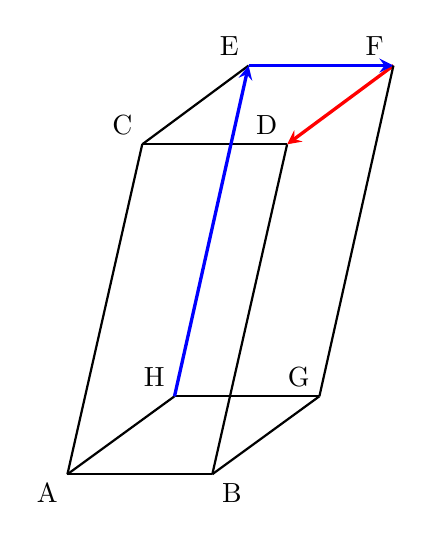
\begin{tikzpicture}[>=stealth]
    \coordinate (A) at (0.35,0.56);
    \coordinate (B) at (2.19,0.56);
    \coordinate (C) at (1.3,4.75);
    \coordinate (D) at (3.14,4.75);
    \coordinate (E) at (2.65,5.75);
    \coordinate (F) at (4.49,5.75);
    \coordinate (G) at (3.55,1.55);
    \coordinate (H) at (1.71,1.55);
    \draw [thick] (A) -- (B);
    \draw [thick] (B) -- (G);
    \draw [thick] (H) -- (G);
    \draw [thick] (H) -- (A);
    \draw [thick] (C) -- (D);
    \draw [very thick, ->, red] (F) -- (D);
    \draw [very thick, ->, blue] (E) -- (F);
    \draw [thick] (E) -- (C);
    \draw [thick] (A) -- (C);
    \draw [thick] (D) -- (B);
    \draw [very thick, ->, blue] (H) -- (E);
    \draw [thick] (F) -- (G);
    \node [below left]  at (A) {A};
    \node [below right] at (B) {B};
    \node [above left]  at (C) {C};
    \node [above left]  at (D) {D};
    \node [above left]  at (E) {E};
    \node [above left]  at (F) {F};
    \node [above left]  at (G) {G};
    \node [above left]  at (H) {H};
\end{tikzpicture}
\end{column}

\begin{column}[t]{0.62\textwidth}
\begin{itemize}
    \item Sejam os vetores \(\vec{AC}\), \(\vec{HG}\) e \(\vec{FD}\)
     \item Vamos calcular \(\vec{AC}+\vec{HG}+\vec{FD}\)
    \item Temos que \(\vec{HG}=\vec{EF}\) (mesma direção, tamanho e sentido)
    \item Temos que \(\vec{AC}=\vec{HE}\) (mesma direção, tamanho e sentido)
    \item Ou seja, podemos trocar \(\vec{AC}\) por \(\vec{HE}\) e \(\vec{HG}\) por \(\vec{EF}\)
    \item \textbf{Ou seja}: 
    \[
    \vec{AC}+\vec{HG}+\vec{FD} = \vec{HE}+\vec{EF}+\vec{FD}
    \]
\end{itemize}
\end{column}
\end{columns}

\end{frame}

\begin{frame}{Exemplo 1}
\begin{columns}

\begin{column}[t]{0.38\textwidth}

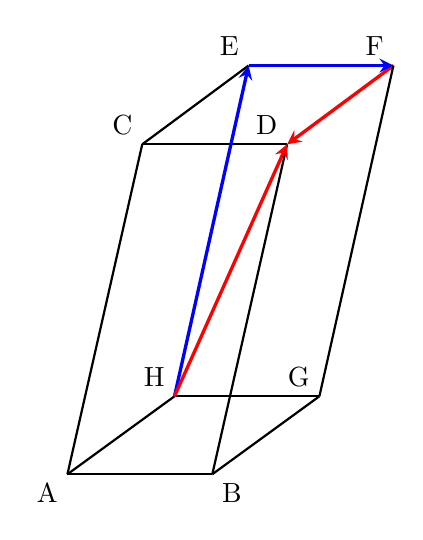
\begin{tikzpicture}[>=stealth]
    \coordinate (A) at (0.35,0.56);
    \coordinate (B) at (2.19,0.56);
    \coordinate (C) at (1.3,4.75);
    \coordinate (D) at (3.14,4.75);
    \coordinate (E) at (2.65,5.75);
    \coordinate (F) at (4.49,5.75);
    \coordinate (G) at (3.55,1.55);
    \coordinate (H) at (1.71,1.55);
    \draw [thick] (A) -- (B);
    \draw [thick] (B) -- (G);
    \draw [thick] (H) -- (G);
    \draw [thick] (H) -- (A);
    \draw [thick] (C) -- (D);
    \draw [very thick, ->, red] (F) -- (D);
    \draw [very thick, ->, blue] (E) -- (F);
    \draw [thick] (E) -- (C);
    \draw [thick] (A) -- (C);
    \draw [thick] (D) -- (B);
    \draw [very thick, ->, blue] (H) -- (E);
    \draw [thick] (F) -- (G);
    \node [below left]  at (A) {A};
    \node [below right] at (B) {B};
    \node [above left]  at (C) {C};
    \node [above left]  at (D) {D};
    \node [above left]  at (E) {E};
    \node [above left]  at (F) {F};
    \node [above left]  at (G) {G};
    \node [above left]  at (H) {H};
    
    \draw[very thick, ->, red] (H) -- (D);
\end{tikzpicture}
\end{column}

\begin{column}[t]{0.62\textwidth}
\begin{itemize}
    \item Sejam os vetores \(\vec{AC}\), \(\vec{HG}\) e \(\vec{FD}\)
    \item Vamos calcular \(\vec{AC}+\vec{HG}+\vec{FD}\)
    \item Temos que \(\vec{HG}=\vec{EF}\) (mesma direção, tamanho e sentido)
    \item Temos que \(\vec{AC}=\vec{HE}\) (mesma direção, tamanho e sentido)
    \item Ou seja, podemos trocar \(\vec{AC}\) por \(\vec{HE}\) e \(\vec{HG}\) por \(\vec{EF}\)
    \item \textbf{Ou seja}: 
    \[
    \vec{AC}+\vec{HG}+\vec{FD} = \vec{HE}+\vec{EF}+\vec{FD}
    \]
    \item Finalmente, temos o vetor \(\vec{HD}\)...
\end{itemize}
\end{column}
\end{columns}

\end{frame}

\begin{frame}{Exemplo 2}
\begin{columns}

\begin{column}[t]{0.38\textwidth}

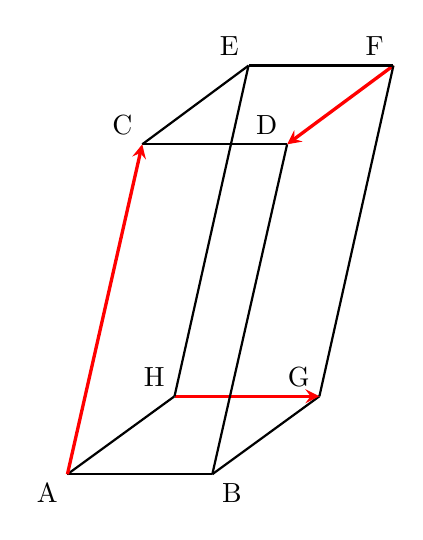
\begin{tikzpicture}[>=stealth]
    \coordinate (A) at (0.35,0.56);
    \coordinate (B) at (2.19,0.56);
    \coordinate (C) at (1.3,4.75);
    \coordinate (D) at (3.14,4.75);
    \coordinate (E) at (2.65,5.75);
    \coordinate (F) at (4.49,5.75);
    \coordinate (G) at (3.55,1.55);
    \coordinate (H) at (1.71,1.55);
    \draw [thick] (A) -- (B);
    \draw [thick] (B) -- (G);
    \draw [very thick, ->, red] (H) -- (G);
    \draw [thick] (H) -- (A);
    \draw [thick] (C) -- (D);
    \draw [very thick, ->, red] (F) -- (D);
    \draw [thick] (F) -- (E);
    \draw [thick] (E) -- (C);
    \draw [very thick,->, red] (A) -- (C);
    \draw [thick] (D) -- (B);
    \draw [thick] (H) -- (E);
    \draw [thick] (F) -- (G);
    \node [below left]  at (A) {A};
    \node [below right] at (B) {B};
    \node [above left]  at (C) {C};
    \node [above left]  at (D) {D};
    \node [above left]  at (E) {E};
    \node [above left]  at (F) {F};
    \node [above left]  at (G) {G};
    \node [above left]  at (H) {H};
\end{tikzpicture}
\end{column}

\begin{column}[t]{0.62\textwidth}
\begin{itemize}
    \item Sejam os vetores \(\vec{AC}\), \(\vec{HG}\) e \(\vec{FD}\)
    \item Vamos calcular \(\vec{AC}-\vec{HG}+\vec{FD}=\vec{AC}+(-\vec{HG})+\vec{FD}\)
    \item Temos que \(-\vec{HG}=\vec{BA}\) (mesma direção, tamanho e sentido oposto ao de \(\vec{HG}\))
    \item Temos que \(\vec{FD}=\vec{GB}\) (mesma direção, tamanho e sentido)
\end{itemize}
\end{column}
\end{columns}

\end{frame}

\begin{frame}{Exemplo 2}
\begin{columns}

\begin{column}[t]{0.38\textwidth}

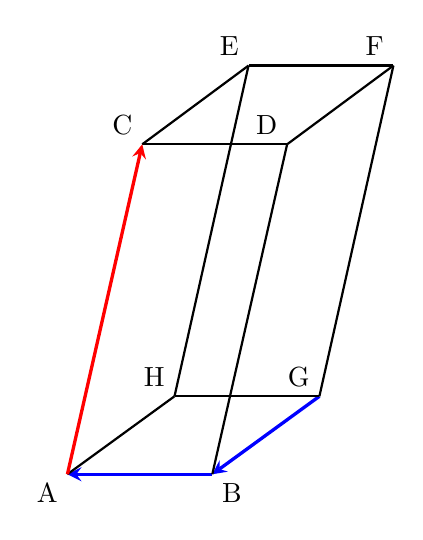
\begin{tikzpicture}[>=stealth]
    \coordinate (A) at (0.35,0.56);
    \coordinate (B) at (2.19,0.56);
    \coordinate (C) at (1.3,4.75);
    \coordinate (D) at (3.14,4.75);
    \coordinate (E) at (2.65,5.75);
    \coordinate (F) at (4.49,5.75);
    \coordinate (G) at (3.55,1.55);
    \coordinate (H) at (1.71,1.55);
    \draw [very thick, <-, blue] (A) -- (B);
    \draw [very thick, <-, blue] (B) -- (G);
    \draw [thick] (H) -- (G);
    \draw [thick] (H) -- (A);
    \draw [thick] (C) -- (D);
    \draw [thick] (F) -- (D);
    \draw [thick] (F) -- (E);
    \draw [thick] (E) -- (C);
    \draw [very thick,->, red] (A) -- (C);
    \draw [thick] (D) -- (B);
    \draw [thick] (H) -- (E);
    \draw [thick] (F) -- (G);
    \node [below left]  at (A) {A};
    \node [below right] at (B) {B};
    \node [above left]  at (C) {C};
    \node [above left]  at (D) {D};
    \node [above left]  at (E) {E};
    \node [above left]  at (F) {F};
    \node [above left]  at (G) {G};
    \node [above left]  at (H) {H};
\end{tikzpicture}
\end{column}

\begin{column}[t]{0.62\textwidth}
\begin{itemize}
    \item Sejam os vetores \(\vec{AC}\), \(\vec{HG}\) e \(\vec{FD}\)
    \item Vamos calcular \(\vec{AC}-\vec{HG}+\vec{FD}=\vec{AC}+(-\vec{HG})+\vec{FD}\)
    \item Temos que \(-\vec{HG}=\vec{BA}\) (mesma direção, tamanho e sentido oposto ao de \(\vec{HG}\))
    \item Temos que \(\vec{FD}=\vec{GB}\) (mesma direção, tamanho e sentido)
    \item Assim: 
    \[
    \vec{AC}+(-\vec{HG})+\vec{FD} = \vec{AC}+\vec{BA}+\vec{GB}
    \]
\end{itemize}
\end{column}
\end{columns}

\end{frame}

\begin{frame}{Exemplo 2}
\begin{columns}

\begin{column}[t]{0.38\textwidth}

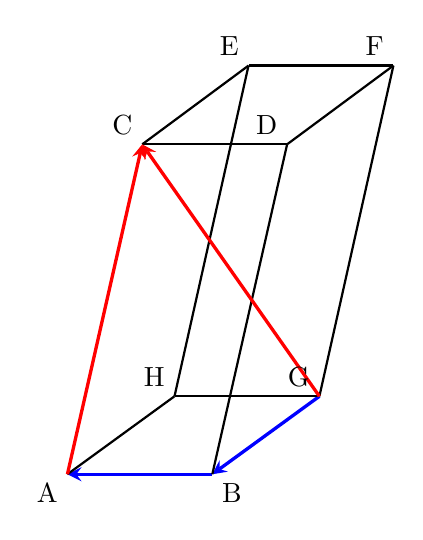
\begin{tikzpicture}[>=stealth]
    \coordinate (A) at (0.35,0.56);
    \coordinate (B) at (2.19,0.56);
    \coordinate (C) at (1.3,4.75);
    \coordinate (D) at (3.14,4.75);
    \coordinate (E) at (2.65,5.75);
    \coordinate (F) at (4.49,5.75);
    \coordinate (G) at (3.55,1.55);
    \coordinate (H) at (1.71,1.55);
    \draw [very thick, <-, blue] (A) -- (B);
    \draw [very thick, <-, blue] (B) -- (G);
    \draw [thick] (H) -- (G);
    \draw [thick] (H) -- (A);
    \draw [thick] (C) -- (D);
    \draw [thick] (F) -- (D);
    \draw [thick] (F) -- (E);
    \draw [thick] (E) -- (C);
    \draw [very thick,->, red] (A) -- (C);
    \draw [thick] (D) -- (B);
    \draw [thick] (H) -- (E);
    \draw [thick] (F) -- (G);
    \draw[very thick,->, red] (G) -- (C);
    \node [below left]  at (A) {A};
    \node [below right] at (B) {B};
    \node [above left]  at (C) {C};
    \node [above left]  at (D) {D};
    \node [above left]  at (E) {E};
    \node [above left]  at (F) {F};
    \node [above left]  at (G) {G};
    \node [above left]  at (H) {H};
\end{tikzpicture}
\end{column}

\begin{column}[t]{0.62\textwidth}
\begin{itemize}
    \item Sejam os vetores \(\vec{AC}\), \(\vec{HG}\) e \(\vec{FD}\)
    \item Vamos calcular \(\vec{AC}-\vec{HG}+\vec{FD}=\vec{AC}+(-\vec{HG})+\vec{FD}\)
    \item Temos que \(-\vec{HG}=\vec{BA}\) (mesma direção, tamanho e sentido oposto ao de \(\vec{HG}\))
    \item Temos que \(\vec{FD}=\vec{GB}\) (mesma direção, tamanho e sentido)
    \item Assim: 
    \[
    \vec{AC}+(-\vec{HG})+\vec{FD} = \vec{AC}+\vec{BA}+\vec{GB}
    \]
    \item Finalmente, temos os vetor \(\vec{GC}\)
\end{itemize}
\end{column}

\end{columns}

\end{frame}


\begin{frame}{Atividade para próxima aula}
    Resolva o exercício 2-10 do livro texto (página 14), explicando os passos utilizados
\end{frame}

